\documentclass[tikz,border=8pt]{standalone}
\usepackage{tikz}
\usetikzlibrary{arrows.meta,positioning}
\begin{document}
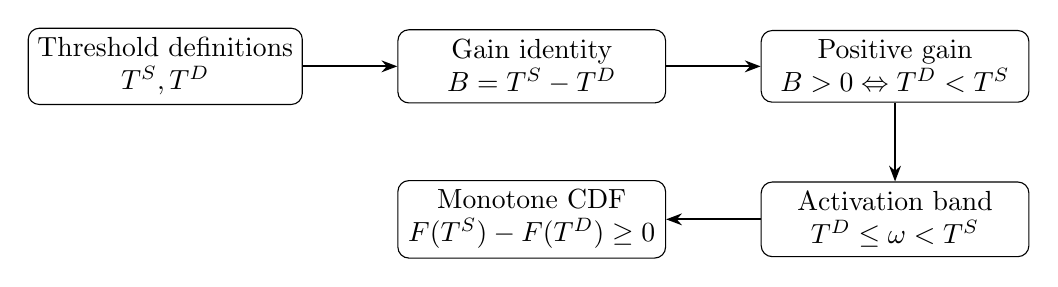
\begin{tikzpicture}[
  node distance=10mm and 12mm,
  box/.style={draw,rounded corners,align=center,minimum width=34mm,minimum height=9mm},
  arr/.style={-{Stealth[length=2mm]},thick}
]
\node[box] (defs) {Threshold definitions\\$T^S, T^D$};
\node[box,right=of defs] (gain) {Gain identity\\$B=T^S-T^D$};
\node[box,right=of gain] (order) {Positive gain\\$B>0 \Leftrightarrow T^D<T^S$};
\node[box,below=of order] (band) {Activation band\\$T^D\leq\omega<T^S$};
\node[box,left=of band] (cdf) {Monotone CDF\\$F(T^S)-F(T^D)\geq0$};
\draw[arr] (defs) -- (gain);
\draw[arr] (gain) -- (order);
\draw[arr] (order) -- (band);
\draw[arr] (band) -- (cdf);
\end{tikzpicture}
\end{document}
